\documentclass{cornell}
\usepackage{lipsum}
\begin{document} 

\title{
    \vspace{-3em}
        \begin{tcolorbox}[colframe=white,opacityback=0]
            \begin{tcolorbox}
                \Huge\sffamily "Introduction to Mathematical Thinking: The Formation of Concepts in Modern Mathematics", WAISMANN, Friedrich. 2003, Dover (first ed - 1959)
            \end{tcolorbox}
        \end{tcolorbox}
    \vspace{-3em}
}
\maketitle

\begin{tcolorbox}
\preread{I read this book in 2015/2016. Even though it self-declares as 'light on formalism', it contains some (heavy) mathematics.}{I wanted to get some insights on the areas inside maths and the main ideas to elaborate proofs and connect missing pieces in different fields. Inspiration for future applications and papers.}
\end{tcolorbox}


\noindent
This book has sixteen chapters and an epilogue. There were some typos in the copy that I purchased at Powell's Books, Portland. The notes below are long and they reflect the huge amount of concepts that I found out in this book. As a personal patterns, I must read the ideas first, take a break, read something similar a few weeks/months later and then come up with insights, inspiration. My brain needs some time to precess and assimilate the new concepts and discussions. 

%\begin{tcolorbox}[colback=white,opacityframe=0]
\topic{Ch. 1 - The various types of numbers}%
{A wide discussion about the natural numbers - they are an ordered system; concept of 'betweeness', predecessor. The introduction of the integers. Fractions (rationals). The concept of dense. We can see an irrational number (√2) as a diagonal of the square. The concept of real numbers. Discussions about the complex numbers and their representation. }%
{OT, I learned a new English word, 'hitherto'}%
%\end{tcolorbox}

\topic{Ch. 2 - Criticism of the Extension of Numbers}%
{Can we simply insert new elements and rules to prove something in Mathematics? This chapter introduces this kind of discussion. Can we create a system where \( 1^x=2 \) ? The idea of 'constructibility'. First examples with geometry}%
{Further reference: H. Hankel; Theory of COmplex Number Systems}%

\topic{Ch. 3 - Arithmetic and Geometry}%
{The 5 axioms from Euclid books. Bolyai and Lobachevsky find a contradiction in the last axiom. The fear of new contradictions in any axiomatic system. The rule association in non-Euclidean and Euclidean geometries. What guarantees the consistency of the Euclidean Geometry? Hilbert helps - 'it it in the theory of real numbers that we must look for the logical foundation of other mathematical system of concepts', including the Euclidean Geometry. How?}%
{Further reference: Pasch, Veronese, Hilbert. Bolyai and Lobachevsky. Klein. Study}%

\topic{Ch. 4 - The Rigorous Construction of the Theory of Integers}%
{'The preservation of the calculating rules governs the concept formation'. This chapter caught my attention - from a single number, we can switch to a distinct representation, using pairs of numbers. That's brilliant! We define Equality, Greater, smaller, sum, difference, multiplication, division.}%
{By introducing the tuples, we allowed subtraction to be performed without restriction - every number couple can be represented as the difference of two positive integers. Diophantine equations and the conclusion that division cannot be performed within the domain of the integers. Sequences and correspondences. Not all the 1-1 relations are isomorphic. The natural numbers are not a subset of the integers! But yes, they have a 1-1, isomorphic correspondence. [Can we extract a subset of correspondences?]}%
{'The negative numbers are greater then ∞ '. The image of ∞ (see \ref{fig01}). We can impress a linear order on the points of a circle - we delete one point and we break the connectedness. We can delete ∞ or zero (ordering of Wallis). The permanence principle - two different orderings for the real numbers; two different number systems. }%
{Further reference: Chuquet, Vieta, Stifel, Wallis, M. Ohm "Perfectly Consistent System of Mathematics"}%

\begin{figure}[!t]
\centering
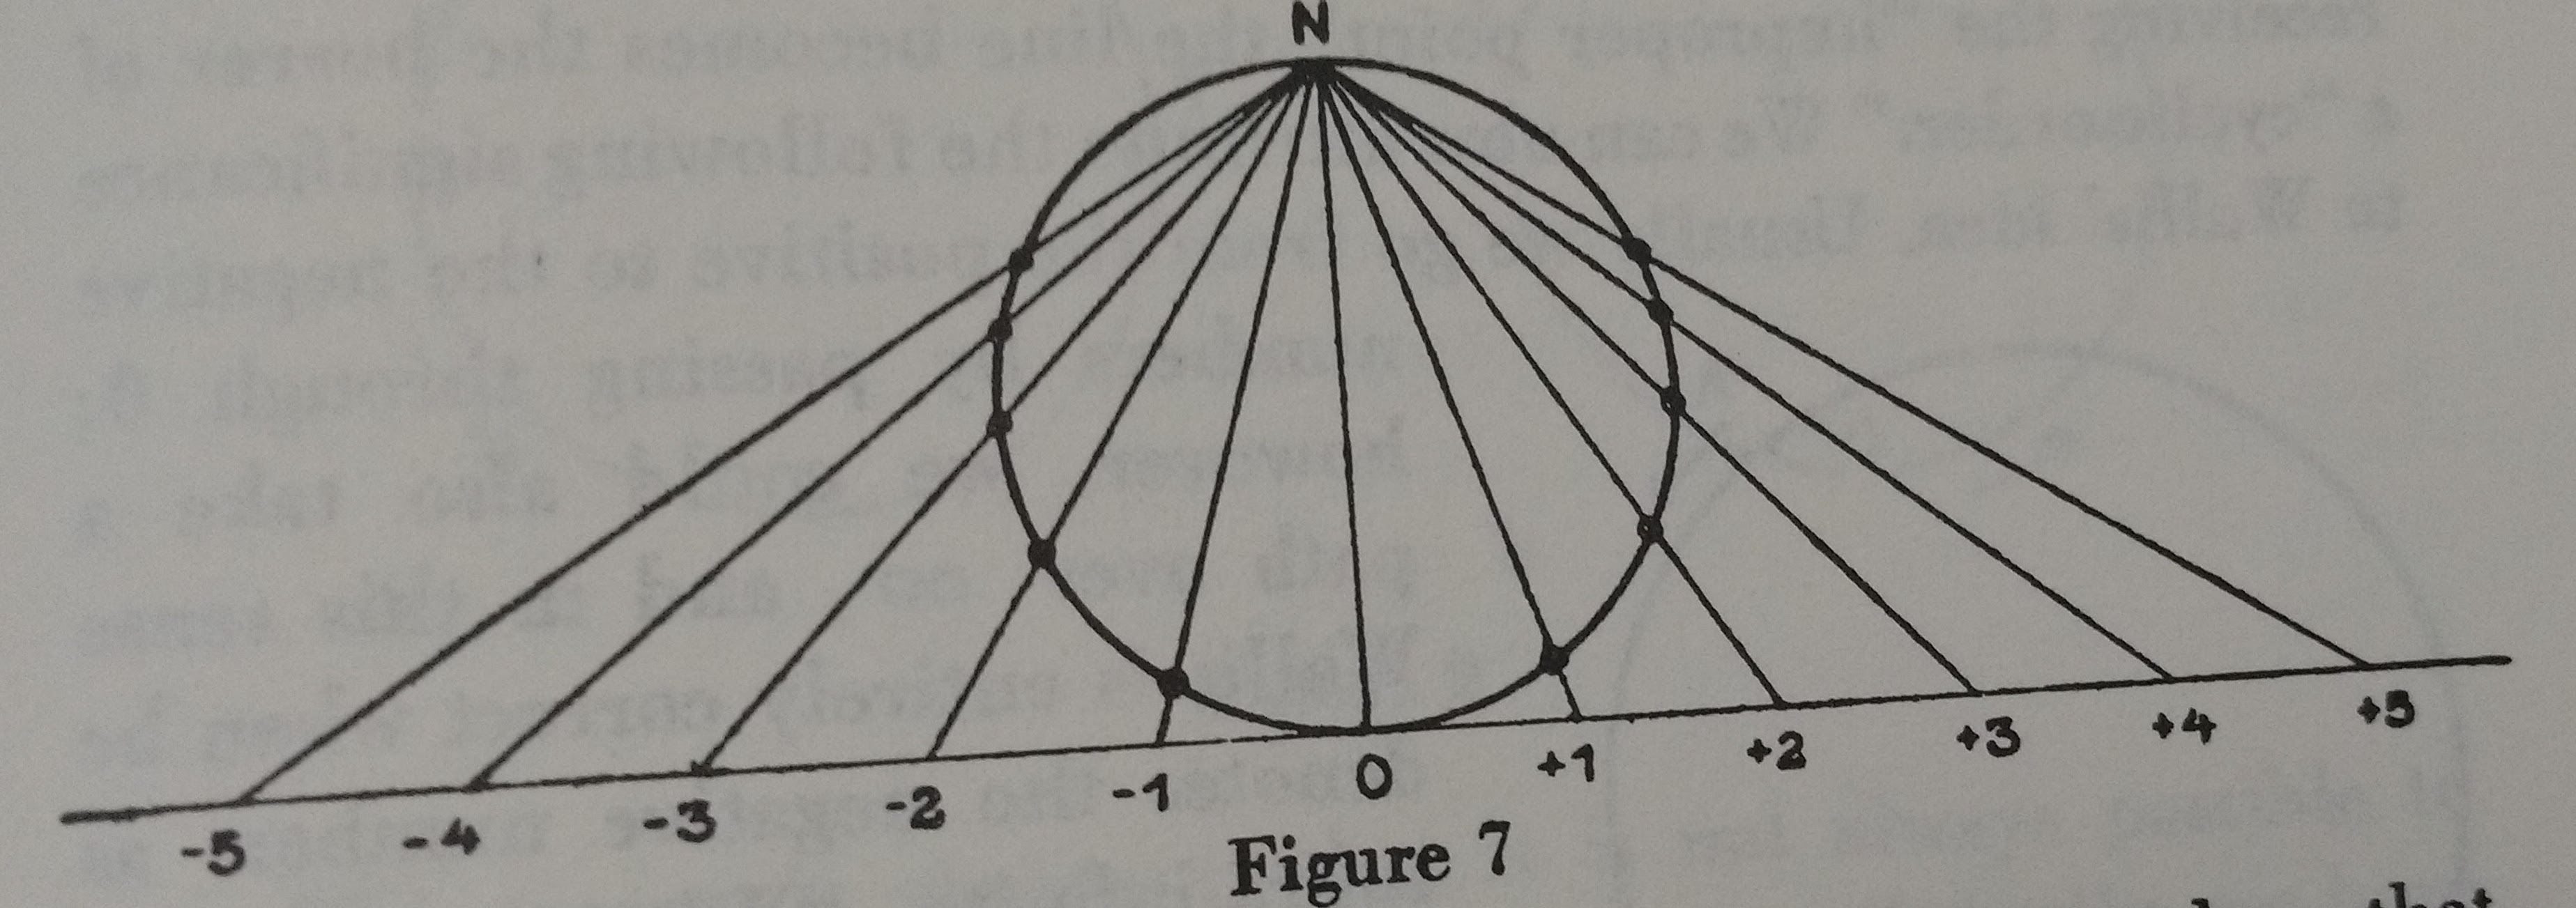
\includegraphics[width=1.0\linewidth]{images/fig001.jpg}
% where an .eps filename suffix will be assumed under latex, 
% and a .pdf suffix will be assumed for pdflatex; or what has been declared
% via \DeclareGraphicsExtensions.
\caption{The image of infinity }
\label{fig01}
\end{figure}

\topic{Ch. 5 - The Rational Numbers}%
{We need a language to do mathematics - Summerian and Akkadian. Interrelation between Maths and languages. [We construct complex thought from sentences, that come from words, that come from syllables. 'We construct the rational numbers with the help of the integers']. Key questions for a system - when are the elements equal? - when is it greater/smaller? - How can we perform operations (add, subtract). Equality on rational numbers. \( ab'b''-a''bb' = 0 \). b' cannot be equals zero; and that means we found a way to exclude the division by zero. AHA! Definition of greater and smaller; associative, commutative, monotony law \( if A > B; A+C>B+C \). Multiplication. "Modulus" (identity) (0 for the sum; 1 for multiplication). The system of integers can be mapped as a part of the rational numbers - 1-1 isomorphic correspondence. The rational numbers are not an extension of the integers. Each of these systems form a closed system. There is a distinction between these elements - 5, +5 and \( \frac{5}{1} \) }%
{Not everything you multiply will be commutative. Experiment of rotating axis in a sphere - the dots may not end up at the same position. NSPQP'; Equator is PQP'. 2 rotations and N - Q or N - P'. Appropriateness and justification. What's a rational number? A: describe the calculus of these numbers. Why do we use tuples? We need the pairs to specify the quotient. What comes first, integers or rationals? [Well... it does not matter.] }%
{Further reference: O. Neugebauer "History of Antique Mathematical Sciences"; CSchlik "Concept of Wholeness"}%

\topic{Ch. 6 - Foundation of the Arithmetic of the Natural Numbers}%
{ Laws for addition and multiplication (considering natural numbers only). Practical computations sum up to the 12 basic laws. The commutative law can be derived from the associative law (Peano 5 basic axioms). Base arithmetic on logic (Frege). Basic concepts of arithmetic = basic logic concepts; arithmetic propositions = predicates. The propositions of logic are tautologies (ex: today is either Mon, Tue, Wed... or Sun; it's always true). Is mathematics a big system of tautologies? No! (Russell shows that maths it's not a tautological system). Theory of types [note to self: this is not type theory]: make sure the elements of a set have a certain homogeneity. Common construction of maths and logic and the axiomatic method. Geometric propositions transferred from one domain to another - isomorphism. Logical calculus - Frege, Russell, Peano. Point, line, plane; we assume combinations of these elements by axioms; it's hard to define them. [Axioms are the initial value; V0, "initial position of the chessman"]. Ask a system of formulas and ask if it's consistent. is there a primitive system, which supports the entire structure of logic and arithmetic? }%
{Further reference: Hamilton and Servois. Stolz. H. Grassmann "Manual or Arithmetic". "The Logical Foundations of Mathematics". König "New Foundations of Logic, Arithmetic and Theory of Sets"}%


\topic{Ch. 7 - Rigorous Construction of Elementary Arithmetic}%
{ Concept of successor \( a+2 = (a+1) +1 or a+2 = succ +1 ; a+3=(a+2)+1 or a+3=(succ+(succ)+1) \) [I created the second interpretation using succ and it reminds of Lisp!]. Recursive definitions. Inference by compete induction. The identity element [and their proofs start with these identity elements). }%

\topic{Ch. 8 - The Principle of Complete Induction}%
{Poincaré - infinity of syllogisms. Frege: "Arithmetic is only an extended logic". Russell: "Mathematical induction is a definition, not a principle." Infinite extension and periodicity: a new type of calculus. Overlapping the abyss of infinite and finite - induction. }%
{Further reference: Dedekind. }%

\topic{Ch. 9- Present Status of the Investigation of the Foundations}%
{Formalism - The problem of Consistency and Gödel: "the consistency of a logical-mathematical system can never be demonstrated by the methods of this system". "Every arithmetic is incomplete". "In every formal system S, a real number can be constructed which cannot be defined in S". Mathematics is a collection of many systems which are mutually closed by the rules of logic and each of which contains problems not decidable within the system itself. It is impossible to distinguish the number series by any inner properties from sequences of another kind.}%
{The Logical School - Attack the problem of defining a number. Sets that are numerically equivalent - 1-1 relation. A number as a class of classes. The number states something about the concept, not about the counted things themselves. What does the command "3 apples!" mean? Frege cannot explain it: the concept of a number is restricted to a subject-predicate from one of the propositions. }%
{Outlook - Some concepts are hard to define, but we know what they mean. "If I am not asked, I know it; if I am asked, I do not know it", and this applies to "What is a number?". The author says that mathematics does not consist of tautologies and it's not a branch of logic, but it contains a series of deductive systems. Logic is a type of calculus. Maths is not one system, but many ones.  }%
{Carnat "The Antinomies and the Incompleteness of Mathematics". G. Gentzen "The Consistency of the Pure Theory of Numbers". Skolem "On Some Questions Regarding the Foundations of Mathematics." Anzhal. H. Schubert. Ramsey, Hahn}%

\topic{Ch. 10 - Limit and point of Accumulation}%
{Series, convergence and limits. The concept of infinity in formulas. "No formula is known by which all the prime numbers can be computed". \( seq: 0,1,0,1,0,1,0.... : a_n = \frac{1}{2}[1+(-1)^n] \) [A binary sequence formula!]. Points of accumulation - some values seem to condense. [Is the idea of a cluster a mathematical construction?]. A limiting point is always a point of accumulation (the converse is not true). A sequence with infinitely many accumulation points. Point of accumulation: every neighbourhood of this point contains infinitely many terms of the sequence. Limit: every neighbourhood of this point contains nearly all the terms of the sequence. Sequences with no point of accumulation, one point of accumulation and many points of accumulation. (convergent sequences \textbf{are not} those with one point of accumulation - HA!) Sequence with infinitely many points of accumulation: the totality of numbers from \( \frac{1}{m}+\frac{1}{n} \), see \ref{fig02}. Sequence where each point is a point of accumulation, see \ref{fig03}. Mechanisms to sum divergent series. [It's important to study sequences; specially for Data Science!]}%
{Further reference: Guido Grandi, Wolff. G. Kowalewski. }%

\begin{figure}[!t]
\centering
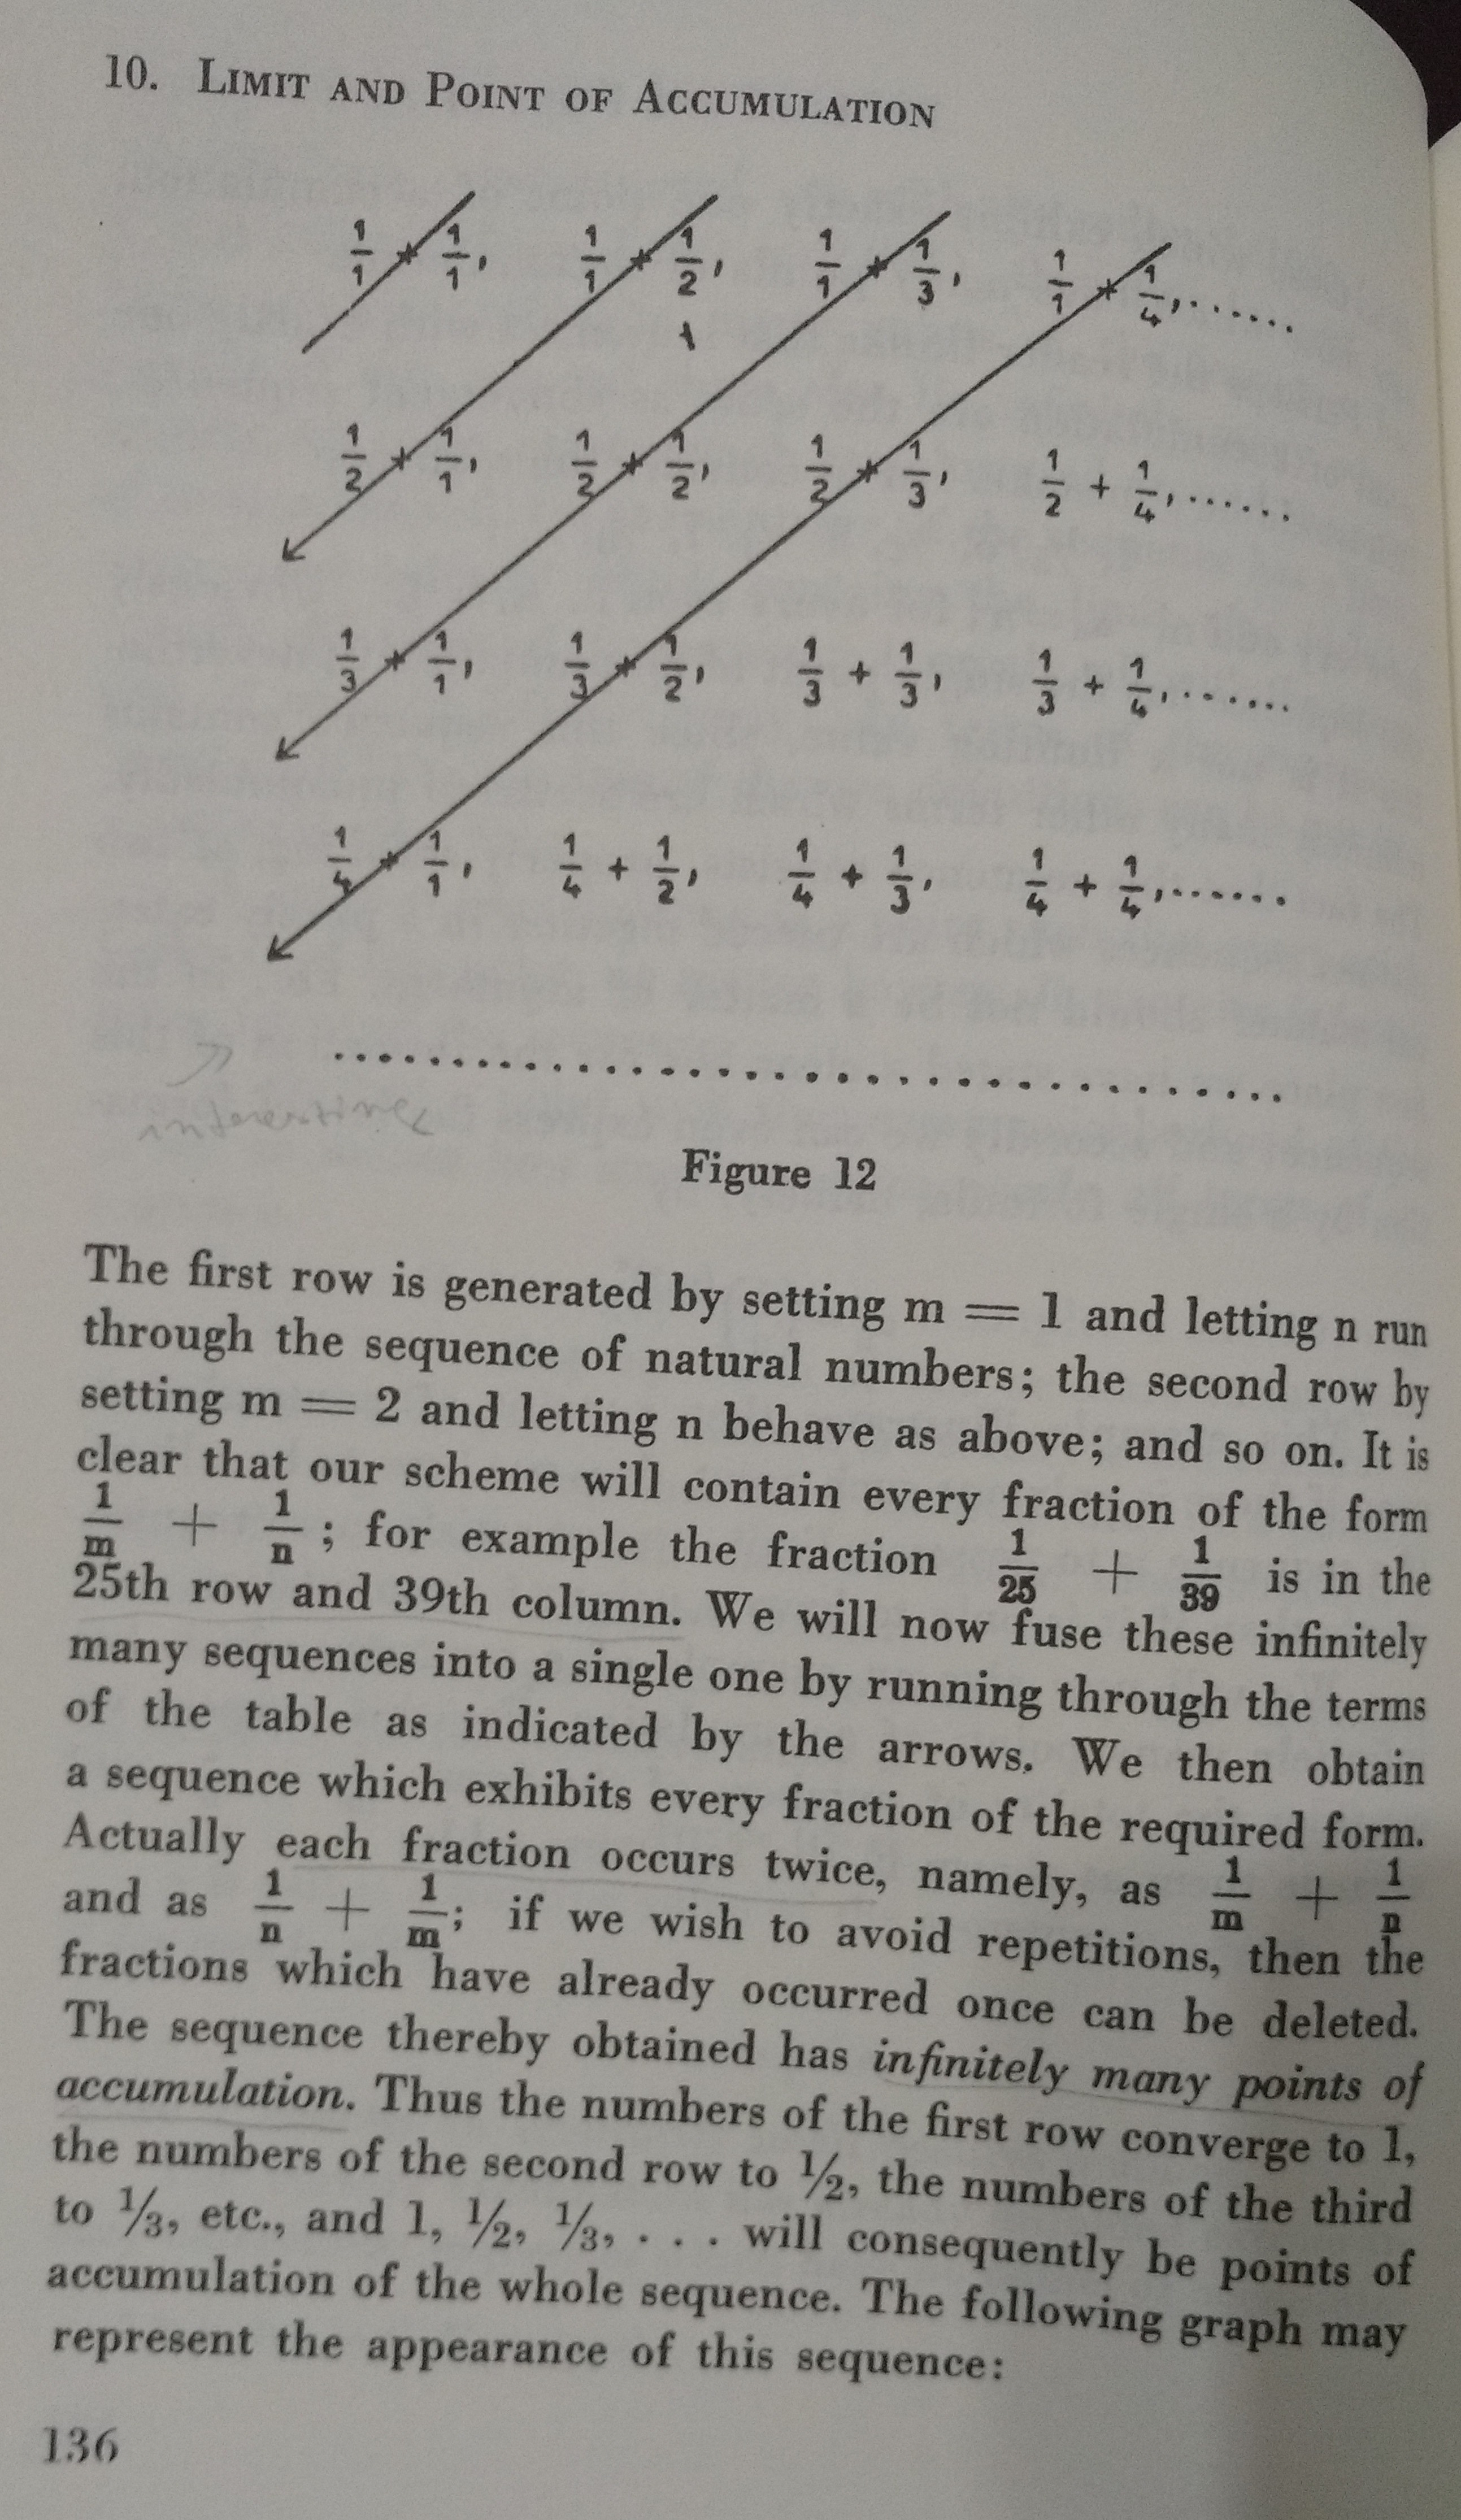
\includegraphics[width=1.0\linewidth]{images/fig002.jpg}
% where an .eps filename suffix will be assumed under latex, 
% and a .pdf suffix will be assumed for pdflatex; or what has been declared
% via \DeclareGraphicsExtensions.
\caption{Sequence with infinitely many points of accumulation }
\label{fig02}
\end{figure}

\begin{figure}[!t]
\centering
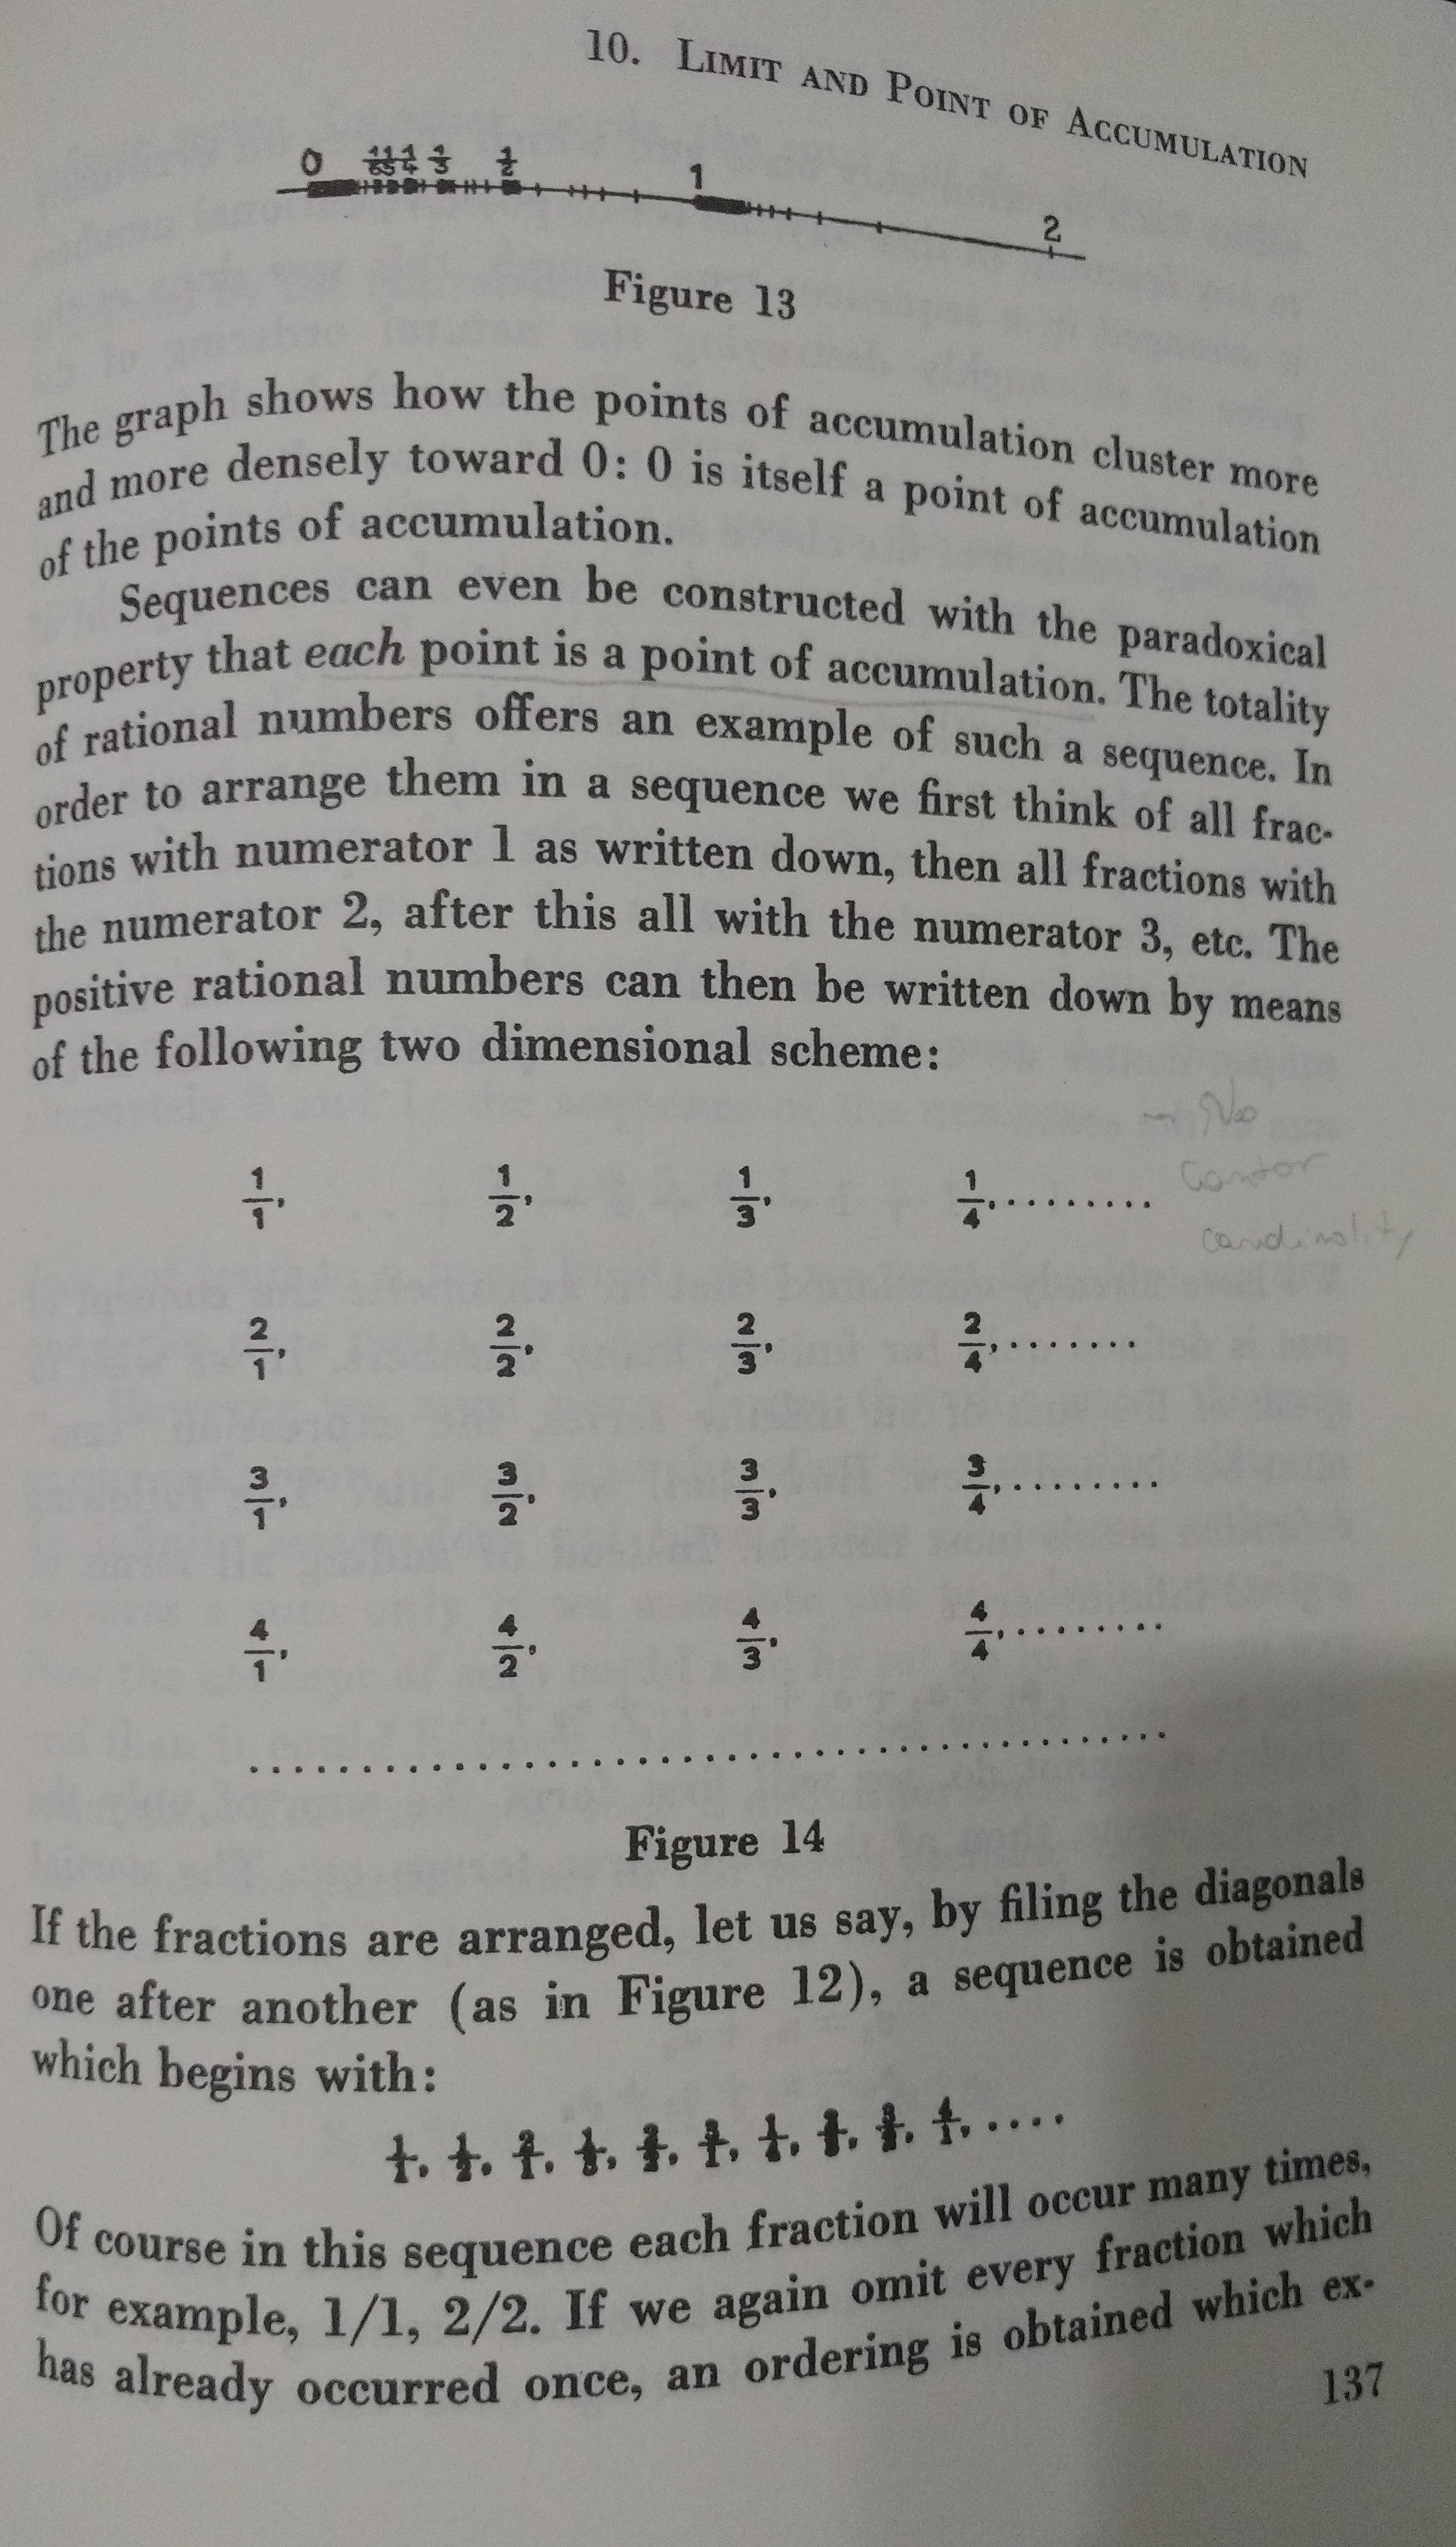
\includegraphics[width=1.0\linewidth]{images/fig003.jpg}
% where an .eps filename suffix will be assumed under latex, 
% and a .pdf suffix will be assumed for pdflatex; or what has been declared
% via \DeclareGraphicsExtensions.
\caption{Sequence where each point is a point of accumulation }
\label{fig03}
\end{figure}

\topic{Ch. 11 - Operating with Sequences. Differential Quotient}%
{The limiting value of a sum of two sequences is equal to the sum of the limiting values of the sequences. Null sequence (converges to zero). The quotient of a null sequence can also be 0 or \( \infty \). Different degrees of smallness. What's the difference between secant and tangent? Instantaneous slope of the curve in a point P. Formal definition of limits and a draft of derivative. Differential quotient \( \frac{dy}{dx} \); it's not a quotient at all, but the limiting value of a sequence of quotients. It's the ratio of the quantities \( \Delta x \Delta y \). An unusual explanation of the chain rule.}%
{Remark: I was quite familiar with the concepts of this chapter, but they were introduced in an unusual way.}%

\topic{Ch. 12 - Remarkable Curves}%
{Wave lines. \( y = \sin\frac{1}{x}\) and . \( y = x\sin\frac{1}{x}\). This curve is continuous at the origin. Weierstrass: There are curves which are continuous everywhere but differentiable nowhere. Koch's curve. Breaking the intuition - not all the continuous functions are differentiable. What is a curve? C. Jordan: a curve is generated if a point runs along in continuous motion. A curve is a continuous and single-valued image of the unit segment (by this definition, a circle would no longer be a curve). There also curves that fill up a square (what???) - Peano and Hilbert showed such concept. Peano's curve [is it differentiable?]. Curves and the distinction between dimensions. Cantor: line segment can be mapped uniquely on a square. The plane (surface) does not contain more points than a line - we can put them into a 1-1 correspondence. What happens with the idea of the part is smaller than the whole? It is true as long as we restrict the question to finite sets!}%
{Peano vs. Cantor: \textbf{Peano}: single-valued in the direction from the line segment to the square (1 pt of the segment, 1 pt of the square); many valued in the direction from the square to the unit segment (1 pt of the square, many pts of the segment); continuous. \textbf{Cantor}: single-valued from the segment to the square; single-valued from the square to the segment; discontinuous. If it's 1-1, it's not continuous. Can we mcreate a structure that satisfies both of these properties, 1-1 and continuous? Jürgens proved that we cannot. Proposition of the invariance of dimensions (Brouwer). "The most characteristic property of curves is their one-dimensionality". A quick mention to topology. What is geometry? "A class of configurations". Projective geometry.Affine geometry. The concept of group (certain systems of operations which are closed in themselves). A group in a system of entities, finite or infinite in number, satisfies 5 conditions: composition, same system, composition is associative, commutativity is not a requirement, unit element (identity), inverse element. Transformation that do not change the elementary-geometric properties of a structure are motions - they form a group called principal group of space transformations. The previous group + parallel projections is the affine group. Affine group + central projections is the projective group. Metric geometry. "Every geometry is a theory of invariants relative to a definite group". The geometry of all 1-1 and continuous point transformations belongs to topology studies, together with the studies of dimensions. 1-1 point transformations and theory of sets. }%
{Remark: unexpected:F. Klein, "Erlanger Programm", it reminds me of the programming language. }%
{Further reference: George Berkeley. Weierstrass. H. v. Koch. Jürgens. Helmholtz. Menger and Urysohn.}%

\topic{Ch. 13 - The Real numbers}%
{Can we formulate the concept of convergence by analysing a sequence of numbers alone whether it converges? Yes. The rational number system is not closed relative to the limit operation. [See the real numbers as a sequence]. Designate sequences as a new kind of number, as a 'real number'. \textbf{Cantor's Theory} null sequence, equality (reflexive, symmetric, transitive). There are infinitely many sequences of numbers which are equal to a given sequence. Greater than (irreflexive, asymmetric, transitive). How are the rational numbers related to the real numbers? Correspondence between the rational numbers and a subclass of sequences. Designate sequence as numbers. To know an irrational number means to know a process for computing it approximately. The irrational number is given only by a construction (a convergent process). An infinite decimal fraction is no more than an abbreviated expression for a nest interval. Every bounded infinite point set has at least one point of accumulation. Every convergent sequence of real number can be replaced by a convergent sequence of rational numbers. \textbf{Dedekind's Theory} There are separations of the rational number in two classes which are not produced by a rational number. The separation has some properties: No class shall be empty; ordering, each entity belongs to only one class. The separation occurs with a cut. An ordered system is continuous if every cut is continuous. There are more cuts in the rational numbers than numbers. Cuts themselves can be interpreted as numbers. Every cut in the domain of real numbers can be replaced by a cut in the domain of the rational numbers. The upper class of a cut is uniquely determined by the lower class. [This is very similar to Russel's ideas and weird constraints]. }%
{Comparison of the two theories above: The structures are defined quite differently. Cantor operates with sequences (nest intervals). Dedekind operates with classes. Dedekind's cut is a kind of condensation of all possible nests of intervals which shrink up to a point. Cantor can handle continua in arbitrary dimensions. In Theory of Sets, the totality of points of accumulation of a set M is called its derived set and it's designated by \( M^1 \). Whe M and \( M^1 \) coincide, we have a perfect set. There are perfect sets which are nowhere dense. The property perfect is not sufficient to characterise the continuity of a straight line. }%
{Uniqueness of the Real Number System - Completeness theorem (ordered system, 4 operations are defined, the system contains a proper subset that can be mapped on the rational numbers by a 1-1, isomorphic correspondence; the Archimedean axiom should be valid). Uniqueness Theorem - every system can be related by a 1-1, isomorphic correspondence, to the system of real numbers. So there's only one system. [The real numbers idea of discontinuity is compatible with quantum mechanics]. The continuum has a different structure. A real number generates extensions, it's not an extension. }%
{Remark: H. Hankel, creator of purely formal theory. Theorem of Bolzano-Weierstrass. Can we fit some of the ideas of ZFC theory as a third comparison? }%
{Further reference: P. du Bois "General Theory of Functions". "Theory of Systems of Complex Numbers".}%

\topic{Ch. 14 - Ultrarreal numbers}%
{Degree of a function; rate of increase. The scale of real numbers might not be enough to designate the order of the poles of a function. Ordinal numbers. Estimation}%
{Remark: Weird, vague chapter. Short one.}%

\topic{Ch. 15 - Complex and Hypercomplex numbers}%
{Imaginary numbers (algebraic and geometric nature - equations and vectors). They helped to establish connections between different parts of mathematics. The function \( \log z \) is infinitely many valued. Gauss: "Analysis is a self-dependent science". Geometrical visualization of the complex numbers. Hamilton: interpret a complex number as a couple of real numbers. [and we go back to the ideas of the initial chapters! Tuples]. Every number couple can be represented as a linear combination of units. There is a subsystem of the complex numbers, where (a, 0) is associated with the system of the real numbers by a 1-1 isomorphism. We cam extend the idea of the complex number to n-tuples (hypercomplex numbers). Quarternions, important to physics (Lorentz transformations and Minkowski). Gauss left some papers with the same ideas. }%
{Further reference: Grassmann}%

\topic{Ch. 16 - Inventing or Discovering?}%
{Abstraction (separation of attributes) or Determination (addition of attributes)? We might not need the general concept of number. Are they invented or discovered? Different ideas. Frege: "Arithmetic can be considered as a game with symbols". Number symbols mean something or not? The geography did not create the rivers; it's the same for mathematics and numbers. Arithmetic is a scince because the numbers exist. The discussions in this chapter are deep and interesting. }%



\summary{There is a one page epilogue. There was too much new information to me in this book. There were no 'Insight' boxes; my brain was busy absorbing the ideas. In general, it was an interesting, challenging book. Some ideas are outdated, but it's interesting to see how the mathematicians behaved in the 50's, just a few years after Russell and Gödel ideas.}



\end{document}